% -*- mode:LaTeX; mode:visual-line; mode:flyspell; fill-column:75 -*-
\section{Introduction}
\label{secIntroduction}


Enabling robots to understand natural language would provide an intuitive interface between lay users and complex robots.
Prior work on enabling robots to understand language has addressed diverse tasks such as following route directions through indoor and outdoor environments or simple manipulation tasks. 

These approaches typically map language to robot plans or high-level symbolic control languages \todo[inline]{FELIX: add some citations here}. This approach is focused solely on high-level reasoning, and assumes that a controller that can adequately execute the plan is available. Hence, natural language has been used mainly as a means of communicating final or intermediate task goals to the robot, but not in specifying \emph{how} to reach those goals. 

Dynamical Systems (DS) based approaches have emerged as an extremely effective means of trajectory representation, which can encapsulate high level \emph{what}'s and lower level \emph{how}'s in a unified representation. Examples of such encodings include \todo[inline]{klas: put some DS citations}. Such DS models are usually tailored to specific tasks via learning from demonstration or reinforcement learning. To the best of our knowledge, NL has previously not been explored in the context of developing DS models for motion representation. 

In this report, we explore NL for online modification of DS models belonging to a recently proposed framework allowing incremental learning in stable DS models \todo[inline]{cite klas's RAS paper}. \todo[inline]{need some sort of example on how the system works from the perspective of the user, e.g. what happens when we say turn left etc.}. We train a model from human demonstrations of the desired behavior modifications (using kinesthetic teaching), and generalize those to novel states in the world.
 During execution, the user can then change the behavior of robot (through the controller) by using the trained natural language commands.








% However, there are many robot tasks that require reasoning not just about \emph{what} to do, but \emph{how} to do it, for example fine manipulation tasks or tasks that require varying impedance during execution.
% To date, no work connects language and robot behavior at the controller\todo{??} level.
% Using a controller such as a Dynamical System provides several key benefits:
% \begin{itemize}
% \item defined over the entire state space: robust to perturbations of the robot.
% \item reactive behavior: robust to perturbations of the environment.
% \item generalizability: a dynamical system provides a family of trajectories, not just a single one.
% \end{itemize}



% In this work, we enable the robot to understand \emph{how} it should do a task using natural language instructions.
% Specifically, we represent a task using a ``vanilla'' DS, and leverage the expressive power of language to infer \emph{modifications} to the Dynamical System.
% We train a model from human demonstrations of the desired behavior modifications (using kinesthetic teaching), and generalize those to novel states in the world.
% During execution, the user can then change the behavior of robot (through the controller) by using the trained natural language commands.




\begin{figure}[t]
  \centering
  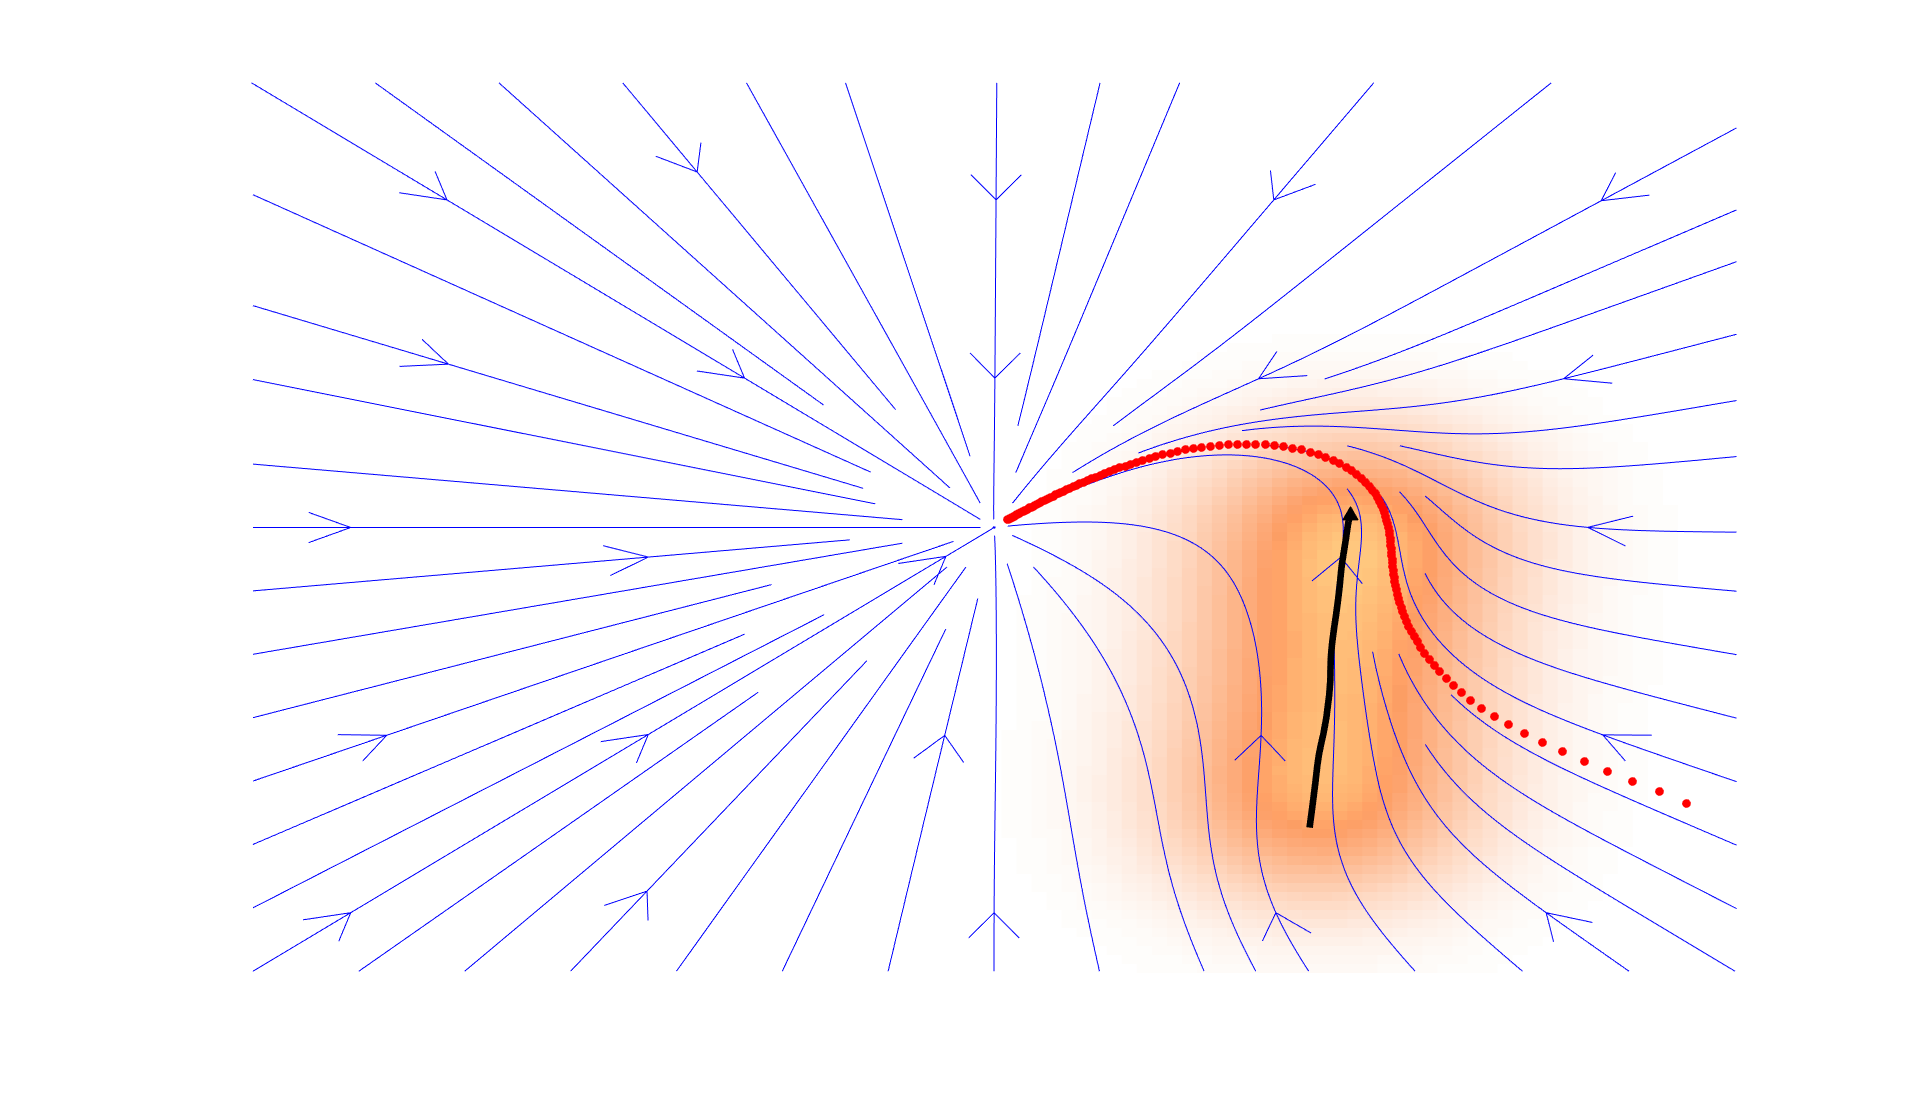
\includegraphics[
    % trim = left bottom right top
    trim = 150mm 50mm 100mm 50mm, clip,
    width = 0.4\textwidth,
  ]{figs/gp_figs/3a-traj1.png}
  \caption{A Modified Dynamical System, representing the controller policy over the entire state space (a 2D plane in this example): at every point the robot follows the gradient until it reaches the attractor.
 In the colored areas, the user has provided a correction to the policy (black arrow), which updates the policy in the same region of state space (re-shaped blue lines).
 This results in a modification to the behavior of the robot (red trajectory).
    Our goal is to use natural language to modify a dynamical system, resulting in a controller that performs the desired behavior.
}
  \label{figProblemSetup}
\end{figure}



% For example, an assistive robot may need to understand how much pressure it should exert when cleaning a patient's skin,
% or a factory robot may need to change how stiffly it should hold a part when cooperatively holding it for a person to assemble,
% or a <> robot may need to know from which direction to approach an object



% attractor point
